\documentclass[a4paper,12pt]{article}
\usepackage[toc,page]{appendix}
\usepackage{listings}
\usepackage{url}
\usepackage{graphicx}
\usepackage[skip=0pt]{caption}
\usepackage{multicol}
\usepackage{float}
\usepackage[margin=1in]{geometry}
%\usepackage{natbib}

\begin{document}

\renewcommand{\thelstlisting}{\thesection.\arabic{lstlisting}}
\renewcommand{\thefigure}{\arabic{section}.\arabic{figure}}
\renewcommand{\thetable}{\arabic{section}.\arabic{table}}
\setlength{\floatsep}{0pt plus 2pt minus 2pt}
%\setlength{\intextsep}{0pt plus 2pt minus 2pt}
%\setlength{\textfloatsep}{0pt plus 2pt minus 2pt}

\title{Introduction to Digital Libraries Assignment \#4}
\date{April 23, 2015}
\author{James Tate II}
\maketitle

\section{Introduction}
Assignment \#4 first required analyzing the changes (if any) in the representations retrieved
in assignment \#3. The same URIs were dereferenced again and compared to the previous
representations. The next part of this assignment involved retrieving TimeMaps of the
analyzed URIs, and analyzing the number of mementos each URI had. The last part of the
assignment required generating graphs of Jaccard Distance over time of 20 URIs.

\section{Methodology}
I wrote several scripts for this assignment and I also modified some previously-written
scripts. They are described in subsections for the different questions in this assginment.

\subsection{Question \#1}
The first part of Question \#1 was to again dereference the URIs that were successfully
processed by boilerpipe in Assignment \#3\cite{hw3}. I used the command in Listing 2-1 to
get a list of the dereferenced URIs that were successfully processed in Assignment \#3.

\begin{lstlisting}[basicstyle=\ttfamily,caption={Getting URIs that
Succeded Boilerpipe Processing }]
    grep -v " 0 " wc_boilerpipe | awk4 \
      | grep -o "\./tweets/[0-9]\+/" \
      > boilerpipe_success_dirs
\end{lstlisting}

Next, I created a new directory to store the second representations of the URIs. I populated
the directory will the URI files I would need to dereference the URIs. These steps are in
Listing 2.2.

\begin{lstlisting}[basicstyle=\ttfamily,caption={Creating Second Tweets Directory}]
    mkdir tweets2
    for i in $(cat boilerpipe_success_dirs);
      do id=$(echo $i | grep -o "[0-9]\+");
      mkdir tweets2/$id;
      cp "${i}url.0" tweets2/$id/url.0;
    done
\end{lstlisting}

I then dereferenced the URIs using the same script from Assignment \#1 which I modified to
used the new directory\cite{hw1}. This step is shown in Listing 2.3. It took 136 seconds to dereference
3035 URIs using 128 parallel processes. 146 did not dereference successfully.

\begin{lstlisting}[basicstyle=\ttfamily,caption={Dereferencing URIs}]
    ./dereference_URIs.py
\end{lstlisting}

After obtaining new representations, I created a list of downloaded represenations and processed the files
with boilerpipe, as shown in Listing 2.4.

\begin{lstlisting}[basicstyle=\ttfamily,caption={Extracting Text with Boilerpipe}]
    find ./tweets2/ > tweets2_file_list
    ./run_boilerpipe.py
\end{lstlisting}

Once I had the textual output from boilerpipe I was ready to start the processing with my \emph{jaccard.py}
script. This script removes most punctuation from the text, generates sets of unigrams, bigrams and trigrams
then calculates the Jaccard Distance between the two representations of each resource\cite{wiki:jaccard}.
These commands to
setup input lists for my script and to run in are in Listing 2.5. The first four commands removed
URIs with a second representation that was not successfuly processed by boilerpipe.

\begin{lstlisting}[basicstyle=\ttfamily,caption={Calculating Jaccard Distance}]
  wc tweets2/*/*/boilerpipe.output | tee wc_boilerpipe2
  grep -v "^ \+0 " wc_boilerpipe | grep -v " total$" \
    | awk4 | grep -o "56[0-9]\+" > boilerpipe1_ids
  grep -v "^ \+0 " wc_boilerpipe2 | grep -v " total$" \
    | awk4 | grep -o "56[0-9]\+" > boilerpipe2_ids
  comm -12 <(sort boilerpipe1_ids) <(sort boilerpipe2_ids) \
    > boilerpipe_common_ids
  ./jaccard.py | tee hw4_report/stats/q1_distances.stats
\end{lstlisting}

The last step for this question was to generate three files for consumption by R to make the graphs in the
Results section. These files were generated by the commands in Listing 2.6.

\begin{lstlisting}[basicstyle=\ttfamily,caption={Generating R Input Files}]
    awk2 q1_distances.stats | tail -n +2 \
      | sort -n > q1_unigrams.stats
    awk3 q1_distances.stats | tail -n +2 \
      | sort -n > q1_bigrams.stats
    awk4 q1_distances.stats | tail -n +2 \
      | sort -n > q1_trigrams.stats
\end{lstlisting}

\subsection{Question \#2}


\subsection{Question \#3}



\section{Results}

\subsection{Question \#1}

\subsection{Question \#2}

\subsection{Question \#3}

\begin{table}[H]
\centering
\caption{Word Count Data}
\begin{tabular}{ | c | c | c | }
\hline
\textbf{Data Point}  & \textbf{Original} & \textbf{After jusText} \\ \hline
Total bytes          & 646,619,835  & 12,133,748    \\ \hline
Total words          & 33,594,568   & 2,035,935     \\ \hline
Unique words         & 9,135,191    & 121,422       \\ \hline
Total letter words   & 81,318,873   & 2,030,636     \\ \hline
Unique letter words  & 1,271,593    & 57,434        \\ \hline
\end{tabular}
\end{table}

%\begin{figure}[H]
%    \centering
%    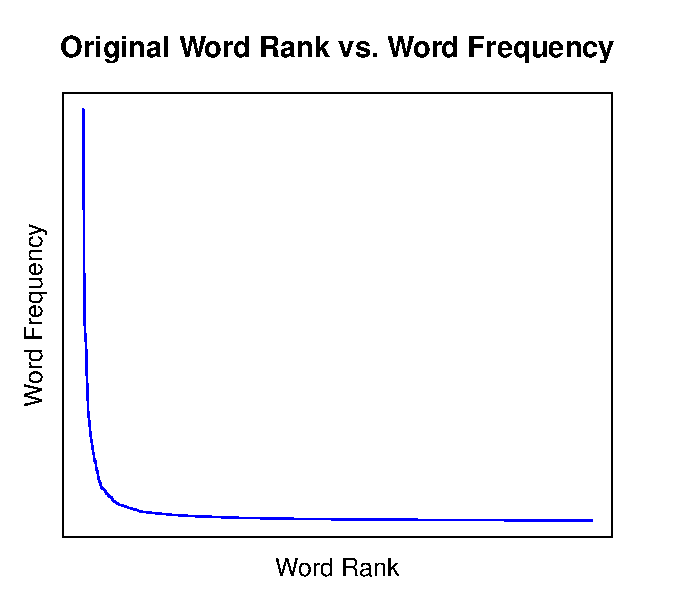
\includegraphics{stats/original_words.pdf}
%    \caption{Rank of Original Words vs. Their Frequency}
%\end{figure}

\bibliographystyle{plain}
\bibliography{../../cs751}

\end{document}
